\documentclass{article}
\usepackage[utf8]{inputenc}

\title{My cool paper on cats!}
\author{Madicken Munk}
\usepackage{hyperref}
\usepackage{multirow}
\usepackage{notoccite}
\hypersetup{colorlinks,
            citecolor=black,
            filecolor=black,
            linkcolor=black,
            urlcolor=black }
\usepackage{graphicx}

\begin{document}

\maketitle

\section{Introduction}
The importance that computational models are verified and validated against
expectations is important to ensure computational predictions are reflective of
expectations. Cats and other animals are often used to train machine learning
algorithms, as it is quite clear from a human perspective if the model is
behaving as one would expect from reality. Kanazawa et al.
\cite{kanazawa_learning_2015} used two-dimensional images of cats to predict how
their bodies move in three-dimensional space. Figure \ref{fig:2dto3dcat}
illustrates their method.


\begin{figure}[h!]
  \centering
  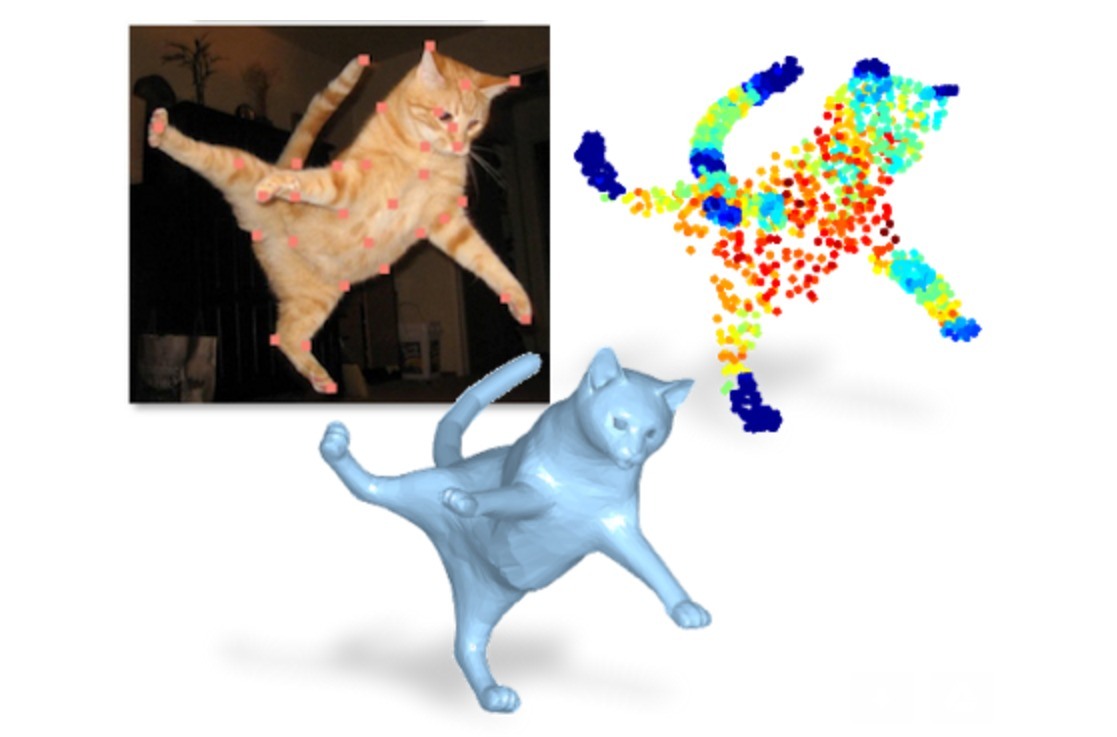
\includegraphics[scale=0.2]{figures/Kanazawa2016}
  \caption{Kanazawa Cats}
  \label{fig:2dto3dcat}
\end{figure}

\section{Conclusion}
Cats are cool!

\bibliographystyle{plain}
\bibliography{bibliography}
\end{document}






